\documentclass[11pt,nocut]{article}

\usepackage{../latex_style/packages}
\usepackage{../latex_style/notations}
\externaldocument{../lecture_02/lecture_02}
\externaldocument{../lecture_04/lecture_04}


\title{\vspace{-2.0cm}%
	Optimization and Computational Linear Algebra for Data Science\\
Lecture 6: Eigenvalues, eigenvectors and Markov chains}
\author{Léo \textsc{Miolane} \ $\cdot$ \ \texttt{leo.miolane@gmail.com}}
\date{\today}

\begin{document}
\maketitle
\textbf{Warning:}
\emph{This material is not meant to be lecture notes. It only gathers the main concepts and results from the lecture, without any additional explanation, motivation, examples, figures...
}


\section{Eigenvalues and eigenvectors}

\begin{definition}\label{def:eigen}
	Let $A \in \R^{n \times n}$. A \textbf{non-zero} vector $v \in \R^n$ is said to be an \emph{eigenvector} of $A$ is there exists $\lambda \in \R$ such that
	$$
	A v = \lambda v.
	$$
	The scalar $\lambda$ is called the eigenvalue (of $A$) associated to $v$. The set
	$$
	E_{\lambda}(A) = \big\{ x \in \R^n \, \big| \, Ax = \lambda x \big\} = \Ker(A-\lambda \Id)
	$$
	is called the eigenspace of $A$ associated to $\lambda$. The dimension of $E_{\lambda}(A)$ is called the multiplicity of the eigenvalue $\lambda$.
\end{definition}

\begin{remark}
	Notice that $E_{\lambda}(A)$ is a subspace of $\R^n$: any (non-zero) linear combination of eigenvectors associated with the eigenvalue $\lambda$ is also an eigenvector of $A$ associated with $\lambda$.
\end{remark}

\begin{remark}
	Definition~\ref{def:eigen} can be generalized to allow complex eigenvalues and eigenvectors: $\lambda \in \C$ and $v \in \C^n$.
	However in this course, we only consider \textbf{real eigenvalues and eigenvectors}. 
\end{remark}

\begin{proposition}
	Let $A \in \R^{n \times n}$. 
	Suppose that $A$ has an eigenvalue $\lambda \in \R$ and let $x \in \R^n$ be an eigenvector associated to $\lambda$.
	The following holds:
	\begin{itemize}
		\item For all $\alpha \in \R$, $\alpha \lambda$ is an eigenvalue of the matrix $\alpha A$ and $x$ is an associated eigenvector.
		\item For all $\alpha \in \R$, $\lambda + \alpha$ is an eigenvalue of the matrix $A + \alpha \Id$ and $x$ is an associated eigenvector.
		\item For all $k \in \N$, $\lambda^k$ is an eigenvalue of the matrix $A^k$ and $x$ is an associated eigenvector.
		\item If $A$ is invertible then $1/\lambda$ is an eigenvalue of the matrix inverse $A^{-1}$ and $x$ is an associated eigenvector.
	\end{itemize}
\end{proposition}

\begin{definition}
	The set of all eigenvalues of $A$ is called the \emph{spectrum} of $A$ and denoted by $\Sp(A)$.
\end{definition}

\begin{proposition}\label{prop:eigen_indep}
	Let $v_1, \dots, v_k$ be eigenvectors of $A$ corresponding (respectively) to the eigenvalues $\lambda_1, \dots, \lambda_k$.
	If the $\lambda_i$ are all distinct ($\lambda_i \neq \lambda_j$ for all $i \neq j$) then the vectors $v_1, \dots, v_k$ are linearly independent.
\end{proposition}

It follows from Proposition~\ref{prop:eigen_indep}:

\begin{corollary}
	A $n \times n$ matrix $A$ admits at most $n$ different eigenvalues: $\# \Sp(A) \leq n$.
\end{corollary}

\section{Diagonalizable matrices}

\begin{definition}[Diagonalizable matrix]
	A matrix $A \in \R^{n \times n}$ is said to be \emph{diagonalizable} if there exists a basis $(v_1, \dots, v_n)$ of $\R^n$ consisting of eigenvectors of $A$, i.e.\ such that there exists $\lambda_1, \dots, \lambda_n \in \R$ such that $Av_i = \lambda_i v_i$.
\end{definition}

For $\lambda_1, \dots, \lambda_n \in \R$, we introduce the notation
$$
\Diag(\lambda_1, \dots, \lambda_n) \defeq
\begin{pmatrix}
	\lambda_1 & 0 & \cdots & 0 \\
	0 & \lambda_2 & & \vdots \\
	\vdots & & \ddots & \vdots \\
	0 & \cdots &  \cdots & \lambda_n
\end{pmatrix} \in \R^{n\times n}.
$$
Notice that $\Diag(\lambda_1, \dots, \lambda_n)$ is diagonalizable, since the canonical basis $(e_1, \dots, e_n)$ is a basis of $\R^n$ consisting of eigenvectors of $\Diag(\lambda_1, \dots, \lambda_n)$.

\begin{proposition}\label{prop:diag}
	A matrix $A \in \R^{n \times n}$ is diagonalizable if and only if there exists an invertible $n \times n$ matrix $P$ and a diagonal matrix $D = \Diag(\lambda_1, \dots, \lambda_n)$ such that
	$$
	A = P D P^{-1}.
	$$
	In this case, the $i^{\rm th}$ column of $P$ is an eigenvector of $A$ associated with the eigenvalue $\lambda_i$.
\end{proposition}

\begin{proposition}
	Let $A = P \Diag(\lambda_1,\dots,\lambda_n) P^{-1}$ (where $P \in \R^{n \times n}$ is invertible) be a diagonalizable matrix. Then
$$
\Tr(A) = \sum_{i=1}^n \lambda_i
\qquad \text{and} \qquad
\rank(A) = \# \{ i \, | \, \lambda_i \neq 0 \}.
$$
Consequently, $A$ is invertible if and only if $\lambda_i \neq 0$ for all $i$. In such case, $A^{-1} = P \Diag(\lambda_1^{-1}, \dots, \lambda_n^{-1}) P^{-1}$.
\end{proposition}

\section{Application to Markov chains}

\subsection{First definitions and properties}

A finite Markov chain is a random process which moves among the elements of a finite set $E$ in the following manner: when at $x \in E$, the next position is chosen according to a fixed probability distribution $P(x, \cdot)$. More formally:

\begin{definition}
	A sequence of random variables $(X_0, X_1, \dots)$ is a Markov chain with state space $E$ and ``transition matrix'' $P$ if for all $t \geq 0$, 
	$$
	\P\big( X_{t+1} = y \, \big| \, X_0= x_0, \dots, X_t = x_t ) = P(x_t,y)
	$$
	for all $x_0, \dots, x_t$ such that $\P(X_0 = x_0, \dots, X_t = x_t) >0$.
\end{definition}

The transition matrix $P$ verifies therefore, for all $x \in E$,
\begin{equation}
	\sum_{y \in E} P(x,y) = 1.
\end{equation}

In order to simplify the notations, we will assume that $E = \{1,2, \dots, n\}$ and write for all $i,j \in E$, $P_{i,j} = P(j,i)$. 
\textbf{Note that we switched here the order of $i$ and $j$. This is not what is usually done in the literature, but this will allow us to be more coherent with our linear algebra framework}.
Such matrix is said to be stochastic:

\begin{definition}[Stochastic matrix]
	A matrix $P \in \R^{n \times n}$ is said to be \emph{stochastic} if:
	\begin{enumerate}[label=(\roman*),noitemsep]
		\item $P_{i,j} \geq 0$ for all $1 \leq i,j \leq n$.
		\item $\sum\limits_{i=1}^n P_{i,j} = 1$, for all $1 \leq j \leq n$.
	\end{enumerate}
\end{definition}

Let $(X_0, X_1, \dots)$ be a Markov chain on $\{1, \dots, n\}$ with transition matrix $P$. For $t \geq 0$ we will encode the distribution of $X_t$ in the vector
$$
x^{(t)} = (x^{(t)}_1, \dots x^{(t)}_n) 
= \big(\P(X_t = 1), \dots, \P(X_t = n)\big) \in \Delta_n
$$
where $\Delta_n$ is the ``$n$-simplex''
$$
\Delta_n \defeq \Big\{ x \in \R^n \, \Big| \, \sum_{i=1}^n x_i = 1 \ \text{and} \ x_i \geq 0 \ \text{for all} \ i \Big\}.
$$


\begin{proposition}
	For all $t \geq 0$
	$$
	x^{(t+1)} = P x^{(t)}
	\quad \text{and consequently,} \quad
	x^{(t)} =  P^t x^{(0)}.
	$$
\end{proposition}
\begin{proof} Let $i \in \{1,\dots, n\}$.
	\begin{align*}
		x^{(t+1)}_i
		= \P(X_{t+1}=i)
		= \sum_{j=1}^n \P(X_{t+1}=i|X_t = j) \P(X_t = j)
		= \sum_{i=1}^n P_{i,j} x^{(t)}_j
		= (Px^{(t)})_i.
	\end{align*}
\end{proof}

\begin{corollary}\label{cor:stab}
	Let $P$ be a stochastic matrix. Then
	\begin{itemize}
		\item For all $x \in \Delta_n$, $Px \in \Delta_n$.
		\item For all $t \geq 1$, $P^t$ is stochastic.
	\end{itemize}
\end{corollary}


\subsection{Invariant measures and the Perron-Frobenius Theorem}

We will be interested in the distribution of $X_t$ for large $t$, that is the limit of $x^{(t)} = P^t x^{(0)}$. As we will see, under suitable conditions on the matrix $P$, $x^{(t)}$ converge to some $\mu \in \Delta_n$ as $t \to \infty$. In such case, by taking the $t \to \infty$ limit in $x^{(t+1)} = P x^{(t)}$ we get $\mu = P \mu$. This motivates the following definition:

\begin{definition}[Invariant measure]
	A vector $\mu \in \Delta_n$ is called an invariant measure for the transition matrix $P$ if $\mu = P \mu$, i.e.\ if $\mu$ is an eigenvector of $P$ associated with the eigenvalue $1$.
	%$$
	%\text{for all} \ j \in \{1, \dots, n\}, \ \mu_i = \sum_{j=1}^n P_{i,j} \mu_j.
	%$$
\end{definition}

%\begin{remark}
	%An invariant measure is an eigenvector of $P$ with associated eigenvalue $1$.
%\end{remark}


\begin{theorem}[Perron-Frobenius, stochastic case]\label{th:perron_frobenius}
	Let $P$ be a stochastic matrix such that there exists $k \geq 1$ such that all the entries of $P^k$ are strictly positive. Then the following holds:
	\begin{enumerate}[label=(\roman*),noitemsep]
		\item\label{item:i} $1$ is an eigenvalue of $P$ and there exists an eigenvector $\mu \in \Delta_n$ associated to $1$.
		\item\label{item:ii} The eigenvectors associated to $1$ are unique up to scalar multiple (i.e.\ $\Ker(P-\Id) = \Span(\mu)$).
		\item\label{item:iii} For all $x \in \Delta_n$, $P^t x \xrightarrow[t \to \infty]{} \mu$.
	\end{enumerate}
\end{theorem}

Theorem~\ref{th:perron_frobenius} is proved in the next section.
Theorem~\ref{th:perron_frobenius} tells us that there is a unique $\mu \in \Delta_n$ such that $P \mu = \mu$. We call $\mu$ the Perron-Frobenius eigenvector of $P$.

\begin{remark}
	There exist a stronger version of the Perron-Frobenius Theorem which does not require the columns of $P$ to sum to $1$, see for instance Theorem~1.1 in \cite{seneta2006non}. The proof is however more involved.
\end{remark}

\begin{corollary}\label{cor:perron}
	Let $P$ be a stochastic matrix such that there exists $k \geq 1$ such that all the entries of $P^k$ are strictly positive. Then there exists a unique invariant measure $\mu$ and for all initial condition $x^{(0)} \in \Delta_n$,
	$$
	x^{(t)} = P^t x^{(0)} \xrightarrow[t \to \infty]{} \mu.
	$$
\end{corollary}

Corollary~\ref{cor:perron} tells us that the Markov chain ``forgets'' its initial condition to converge to its invariant measure $\mu$. We say that the chain is ``mixing''. 
\\

Working a little bit more, one can prove the ``ergodic'' Theorem that states that $\mu_i$ corresponds to the average time spent by the Markov chain in state $i$.

\begin{theorem}[Ergodic Theorem]\label{th:ergodic}
	Let $(X_t)_{t \geq 0}$ be a Markov chain whose transition matrix is $P$.
	Assume that there exists $k \geq 1$ such that all the entries of $P^k$ are strictly positive and let $\mu$ be the unique invariant measure of $P$. Then for any initial condition $X_0$, we have with probability $1$, for all $i=1, \dots, n$:
	$$
	\frac{1}{T} \# \big\{ t < T \, \big| \, X_t = i \big\}
	\xrightarrow[T \to \infty]{} \mu_i.
	$$
\end{theorem}


\subsection{Proof of Theorem~\ref{th:perron_frobenius}}
We first prove the theorem in the case $k=1$, when $P_{i,j} > 0$ for all $i,j$.
\begin{lemma}\label{lem:contract}
	The mapping 
	$$
	\begin{array}{cccc}
		\varphi:& \Delta_n &\to& \Delta_n \\
				& x & \mapsto & Px
	\end{array}
	$$
	is contracting for the $\ell_1$-norm: there exists $c \in (0,1)$ such that for all $x,y \in \Delta_n$:
	$$
	\| Px - Py \|_1 \leq c \| x-y\|_1.
	$$
\end{lemma}
\begin{proof}
	%Let $x \in \Delta_n$. Since the entries of $x$ and $P$ are non-negative, the entries of $Px$ are also non-negative. Compute
	%$$
	%\|Px\|_1 = \sum_{i=1}^n (Px)_i = \sum_{i=1}^n \sum_{j=1}^n P_{i,j} x_j
	%= \sum_{j=1}^n \Big(\sum_{i=1}^n P_{i,j}\Big) x_j.
	%$$
	%Since $P$ is stochastic  we have $\sum_{i=1}^n P_{i,j} = 1$ which gives
	%$$
	%\|Px\|_1 = \sum_{j=1}^n x_j = 1.
	%$$
	%Hence $Px \in \Delta_n$. 
	First notice that $\varphi$ is well-defined by Corollary~\ref{cor:stab}.
	Let us write $\alpha \defeq \min_{i,j} P_{i,j} \in (0,1)$.
	Let $x,y \in \Delta_n$. We will show that $\| Px - Py \|_1 \leq (1-\alpha) \| x-y\|_1$, i.e.\ $\|P z\|_1 \leq \alpha \|z\|_1$ where $z = x-y$. Compute
	$$
	\| P z\|_1 
	= \sum_{i=1}^n \big| (Pz)_i \big|
	= \sum_{i=1}^n \Big| \sum_{j=1}^n P_{i,j}z_j \Big|.
	$$
	Since $\sum_{j} z_j = 0$ we have $\sum_j (P_{i,j} - \alpha/n) z_j = \sum_j P_{i,j} z_j$. Hence
	$$
	\| P z\|_1 
	= \sum_{i=1}^n \Big| \sum_{j=1}^n (P_{i,j} - \alpha/n) z_j \Big|
	\leq \sum_{i=1}^n \sum_{j=1}^n (P_{i,j} - \alpha/n) |z_j| 
	= \sum_{j=1}^n (1-\alpha) |z_j|
	= (1-\alpha) \|z\|_1.
	$$
\end{proof}

Using Lemma~\ref{lem:contract}, Banach fixed point Theorem tells us that $\varphi$ admits a unique fixed point $\mu$ on $\Delta_n$ (i.e.\ a unique $\mu \in \Delta_n$ such that $P\mu = \mu$) and that for all $x \in \Delta_n$, $P^t x \xrightarrow[t \to \infty]{} \mu$. This proves Theorem~\ref{th:perron_frobenius} in the case $k=1$.
\\

In the case $k > 1$ we simply apply the result for $k=1$ to $P^k$.
This gives that there exists a unique $\mu \in \Delta_n$ such that $P^k \mu = \mu$. Multiplying by $P$ on both sides leads to $P^k (P\mu) = P\mu$. 
Since $P\mu \in \Delta_n$ we obtain that $P\mu = \mu$ by uniqueness of $\mu$. This proves~\ref{item:i}. To prove~\ref{item:ii} we consider $x \in \R^n$ such that $P x = x$. By iteration we get $P^k x = x$ which implies (using the result on $P^k$) that $x \in \Span(\mu)$.
To prove~\ref{item:iii} we fix $\ell \in \{0, \dots, k-1\}$. Let $x \in \Delta_n$. By applying the point~\ref{item:iii} to $P^k$, we have 
$$
P^{kt} P^{\ell} x \xrightarrow[t \to \infty]{} \mu.
$$
Since this holds for all $\ell \leq k-1$ we obtain that $P^r x \xrightarrow[r \to \infty]{} \mu$ using the Euclidean division of $r$ by $k$.

\section{Example: Google's PageRank algorithm}

\subsection{The PageRank algorithm}

The PageRank algorithm was invented by Larry Page and Sergey Brin \cite{page1999pagerank}.
The goal is to rank $n$ web pages in terms of ``importance''.
L.\ Page and S.\ Brin  considered a ``drunk surfer'' that goes from a page $j$ to an other page $i$ by randomly clicking on the links that are on the page $j$.
This can be modeled by a Markov chain with state space $\{1, \dots, n\}$ and transition matrix $P$ given by
$$
P_{i,j} 
= 
\begin{cases}
	1 / \deg(j) & \text{if there is a link} \ j \to i \\
	0 & \text{otherwise},
\end{cases}
$$
where $\deg(j)$ denotes the number of outgoing links on page $j$.
The idea behind PageRank is to quantify the importance of a page $i$ by the fraction of time spent by the ``drunk surfer'' on it. By Theorem~\ref{th:ergodic} we know that this corresponds to the coefficient $\mu_i$ of the invariant measure $\mu$ of $P$.
\\

The matrix $P$ is however not guaranteed to satisfy the hypotheses of Theorem~\ref{th:ergodic}-Corollary~\ref{cor:perron}. Brin and Page proposed to use instead of $P$ the matrix
$$
G = \alpha P + \frac{1-\alpha}{n} \1,
$$
where $\alpha \in (0,1)$ is a parameter close to $1$ (Google takes $\alpha \simeq 0.85$) and $\1$ denotes the all-one matrix.
The PageRank algorithm computes $\mu$ the Perron-Frobenius eigenvector of the matrix $G$ and ranked the webpages according to their coordinate in the vector $\mu$: the higher $\mu_i$, the better page $i$ will be ranked.

\subsection{Ranking tennis players}

The ideas behind PageRank can be applied in many different contexts, not only for ranking webpages.
In the following example we aim at ranking the following $n=54$ tennis players:
\begin{center}
Federer, Nadal, Djokovic, Murray, Del Potro, Roddick, Coria, Zverev, Ferrer, Soderling, Tsonga, Nishikori, Raonic, Nalbandian, Wawrinka, Berdych, Hewitt, Tsitsipas, Monfils, Gonzalez, Thiem, Ljubicic, Davydenko, Cilic, Pouille, Safin, Isner, Dimitrov, Medvedev, Ferrero, Goffin, Bautista Agut, Sock, Gasquet, Simon, Blake, Monaco, Coric, Stepanek, Khachanov, Almagro, Robredo, Verdasco, Anderson, Youzhny, Baghdatis, Dolgopolov, Kohlschreiber, Fognini, Melzer, Paire, Querrey, Tomic, Basilashvili.
\end{center}

To do so, we have access to the ``head to head'' record between them (see Figure~\ref{fig:confrontations}) in the form of the matrix $R \in \R^{n \times n}$:
\begin{equation}\label{eq:def_R}
R_{i,j} = \ \text{<<\,number of wins of player $i$ against player $j$\,>>}.
\end{equation}


We will use the PageRank strategy of the previous section in order to rank the players. In our case, instead of a ``drunk surfer'' we will consider a ``drunk spectator''.
At time $t$ the value $X_t \in \{1, \dots, n\}$ indicates which tennis player the spectator believes to be the best. At time $t+1$, the spectator picks uniformly at random a game played by its favorite player $X_t$ against one of the other players, $x$.
If the game was won by $X_t$, then the spectator still believes that $X_t$ is the best: $X_{t+1} = X_t$. Otherwise the spectator changes his mind: $X_{t+1} = x$.

This can be modeled by a Markov chain with transition matrix:
$$
P_{i,j} = 
\begin{cases}
	V_j/G_j & \text{if} \ i = j \\
	R_{i,j}/G_j & \text{otherwise,}
\end{cases}
$$
where $V_j$ denotes the total number of victories of player $i$ and where $G_j$ denotes the total number of game played by $j$:
$$
V_{j} = \sum_{i=1}^n R_{j,i} \qquad \text{and} \qquad G_j = \sum_{i=1}^n R_{i,j} + R_{j,i}.
$$
Let $\mu$ be the ``Perron-Frobenius'' eigenvector of $P$. The vector $\mu$ is displayed on Figure~\ref{fig:ranking}.
Applying Corollary~\ref{cor:perron}-Theorem \ref{th:ergodic} to the matrix $P$ we get that the ``drunk spectator'' will (in the $t \to \infty$ limit) spend a fraction $\mu_i$ of its time thinking that the player $i$ is the best. The values $(\mu_1, \dots, \mu_n)$ can therefore be used to rank the players. We obtain the following order (see also Figure \ref{fig:ranking})
\begin{center}
Federer (14.4\%),
Djokovic (13.7\%),
Nadal (13.6\%),
Murray (5.8\%),
Ferrer (3.0\%),
Del Potro (2.8\%),
Berdych (2.5\%),
Roddick (2.4\%),
Wawrinka (2.3\%),
Tsonga (2.1\%),
Nishikori (1.6\%),
Nalbandian (1.6\%),
Hewitt (1.5\%),
Monfils (1.5\%),
Davydenko (1.5\%),
Cilic (1.4\%),
Soderling (1.4\%),
Verdasco (1.2\%),
Gonzalez (1.2\%),
Raonic (1.2\%),
Ljubicic (1.2\%),
Gasquet (1.2\%),
Simon (1.1\%),
Thiem (1.1\%),
Isner (1.0\%),
Zverev (1.0\%),
Youzhny (1.0\%),
Robredo (0.9\%),
Kohlschreiber (0.9\%),
Ferrero (0.9\%),
Stepanek (0.8\%),
Safin (0.8\%),
Dimitrov (0.8\%),
Almagro (0.7\%),
Baghdatis (0.7\%),
Blake (0.7\%),
Anderson (0.7\%),
Goffin (0.7\%),
Coria (0.7\%),
Bautista Agut (0.6\%),
Monaco (0.6\%),
Fognini (0.6\%),
Querrey (0.6\%),
Melzer (0.6\%),
Dolgopolov (0.5\%),
Coric (0.5\%),
Pouille (0.4\%),
Tsitsipas (0.4\%),
Sock (0.4\%),
Paire (0.3\%),
Medvedev (0.3\%),
Khachanov (0.3\%),
Tomic (0.2\%),
Basilashvili (0.1\%).
\end{center}

\begin{figure}[h!]
    \centering
	\hspace*{-2cm}
	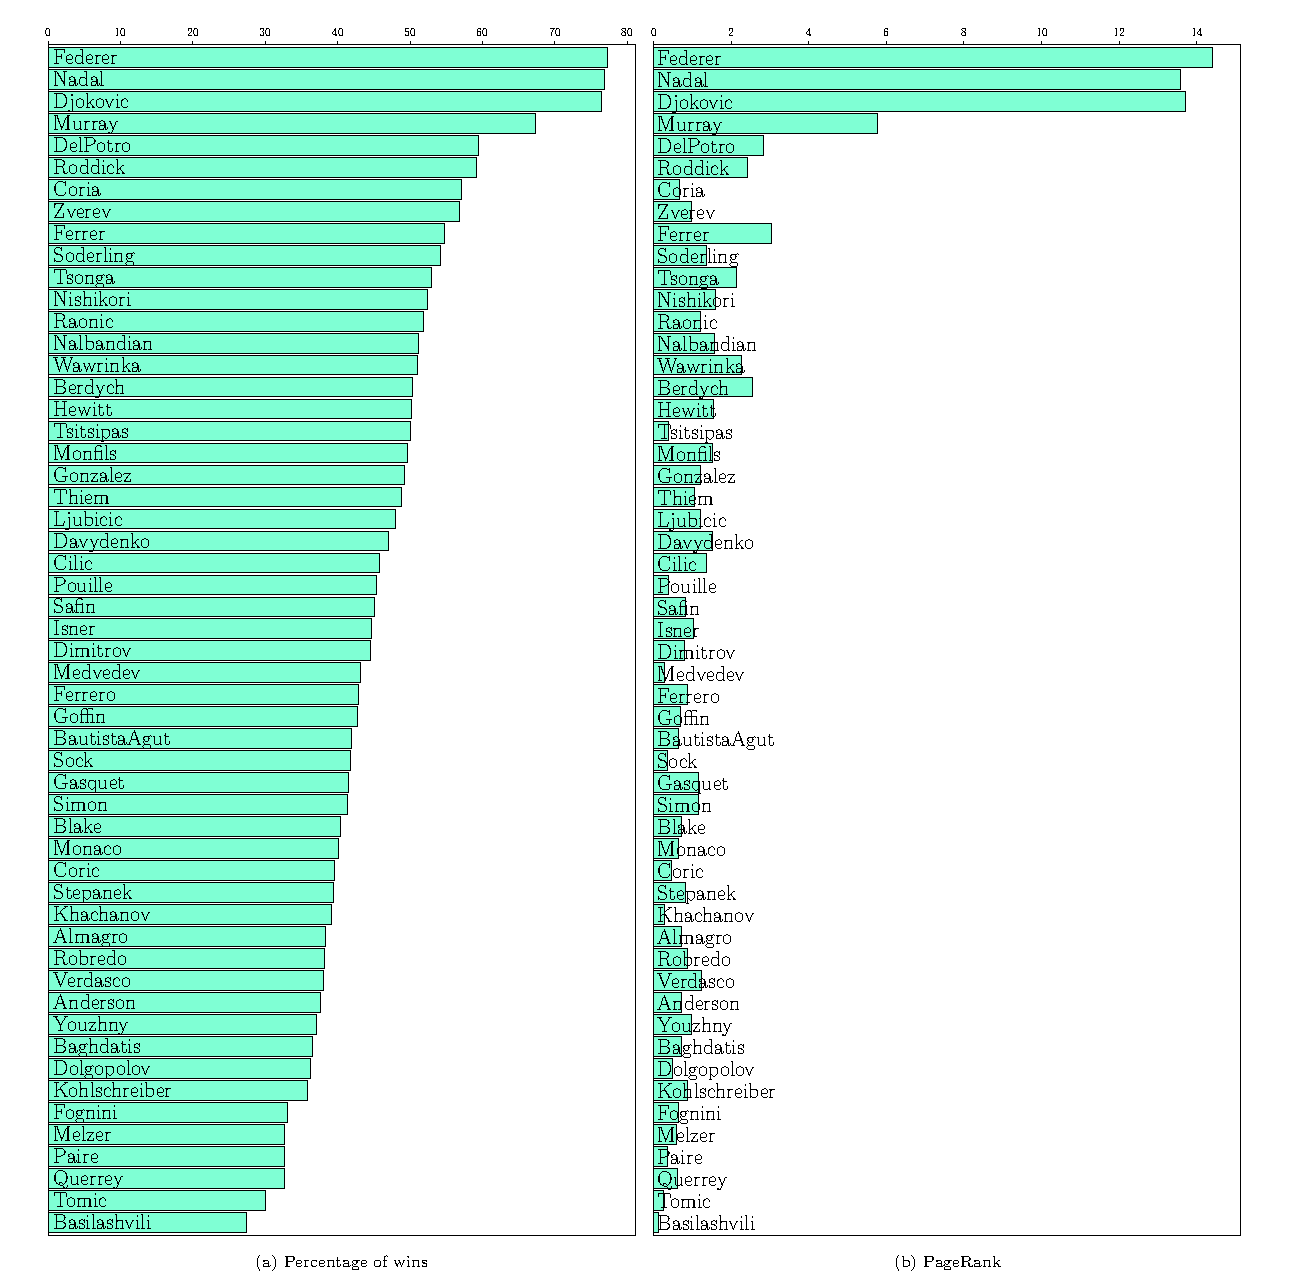
\includegraphics[width=1.23\textwidth]{./pagerank_tennis.pdf}
	\caption{Comparison of the ranking by the percentage of wins (on the left) and the ranking using PageRank.}
	\label{fig:ranking}
\end{figure}
\begin{figure}[h!]
    \centering
	\hspace*{-2cm}
	
\includegraphics[width=1.23\textwidth]{./confrontations.pdf}
	\caption{The matrix $R$ given by \eqref{eq:def_R}}
	\label{fig:confrontations}
\end{figure}


\vspace{1cm}
\centerline{\pgfornament[width=7cm]{71}}


\bibliographystyle{plain}
\bibliography{../references.bib}
\end{document}
